\section{Quantum Mechanics Foundations}
\label{sec:quantum-foundations}

This section establishes the quantum mechanical principles that underpin quantum automata theory. We emphasize both the mathematical formalism and the conceptual distinctions from classical systems. In what follows, we review the basic postulates of quantum mechanics, elaborate on the structure and evolution of quantum states, and discuss measurement, decoherence, and their computational implications.



\subsection{Qubits and Quantum States}
\label{subsec:qubits}

\begin{definition}[Qubit]
A \emph{\gls{qubit}} is the fundamental unit of quantum information. It is represented as a normalised vector in a two-dimensional complex Hilbert space,
\[
\mathcal{H} = \mathbb{C}^2.
\]
\end{definition}

\begin{notation}[Computational Basis]
The standard (computational) basis states for a qubit are defined as
\[
|0\rangle = \begin{pmatrix} 1 \\ 0 \end{pmatrix}, \quad |1\rangle = \begin{pmatrix} 0 \\ 1 \end{pmatrix}.
\]
\end{notation}

\begin{definition}[General Qubit State]
A general state of a \gls{qubit} is given by
\[
|\psi\rangle = \alpha|0\rangle + \beta|1\rangle, \quad \text{with } |\alpha|^2 + |\beta|^2 = 1,
\]
where \(\alpha,\beta \in \mathbb{C}\) are the \emph{probability amplitudes}.
\end{definition}

\begin{remark}
Global phase factors—i.e. multiplying the state by an overall phase \(e^{i\gamma}\)—do not affect the physical properties of the qubit.
\end{remark}

\begin{example}[Bloch Sphere Representation]
  Any pure state of a \gls{qubit} can be written in the form
  \[
  |\psi\rangle = \cos\frac{\theta}{2}|0\rangle + e^{i\phi}\sin\frac{\theta}{2}|1\rangle,
  \]
  with \(\theta \in [0,\pi]\) and \(\phi \in [0,2\pi)\). Figure~\ref{fig:bloch_sphere} illustrates the \textbf{Bloch sphere} representation of a qubit \cite{nielsen2010quantum}.
\end{example}

\begin{figure}[h]
  \centering
  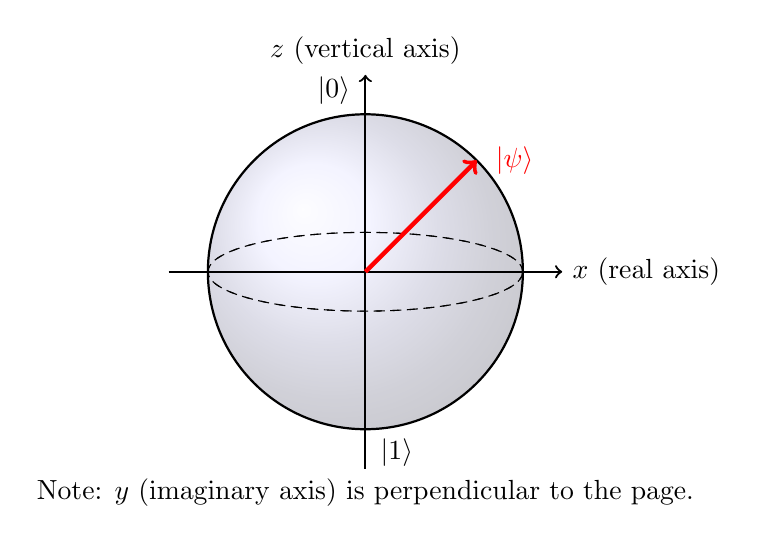
\begin{tikzpicture}[scale=1]
    % Draw sphere outline with shading
    \shade[ball color=blue!20, opacity=0.3] (0,0) circle (2cm);
    \draw[thick] (0,0) circle (2cm);
    
    % Draw equator as a dashed ellipse (horizontal cross-section)
    \draw[dashed] (0,0) ellipse (2cm and 0.5cm);
    
    % Draw meridian arcs (vertical cross-sections)
    \draw[dashed] (-2,0) arc (180:0:2cm and 0.5cm);
    \draw[dashed] (2,0) arc (0:-180:2cm and 0.5cm);
    
    % Axes: x and z
    \draw[->, thick] (-2.5,0) -- (2.5,0) node[right] {$x$ (real axis)};
    \draw[->, thick] (0,-2.5) -- (0,2.5) node[above] {$z$ (vertical axis)};
    
    % Mark north and south poles with horizontal shift
    \node[above, xshift=-0.4cm] at (0,2) {\(|0\rangle\)};
    \node[below, xshift=0.4cm] at (0,-2) {\(|1\rangle\)};
    
    % Bloch vector in the x-z plane
    \draw[->, red, ultra thick] (0,0) -- (1.414,1.414) node[right] {\(\;|\psi\rangle\)};
    
    % Note for y axis
    \node at (0,-2.8) {Note: \(y\) (imaginary axis) is perpendicular to the page.};
  \end{tikzpicture}
  \caption{Enhanced Bloch sphere representation of a \gls{qubit} with adjusted labels.}
  \label{fig:bloch_sphere}
  \end{figure}

\begin{observation}
  For multi-qubit systems, the overall state space is given by the tensor product of individual qubit spaces. For instance, a two-qubit system is described by
  \[
  |\psi\rangle = \sum_{i,j \in \{0,1\}} \alpha_{ij}\, |i\rangle \otimes |j\rangle, \quad \sum_{i,j} |\alpha_{ij}|^2 = 1.
  \]
  This exponential scaling of the state space underpins the potential of quantum parallelism \cite{nielsen2010quantum}.
\end{observation}



\subsection{Superposition and Entanglement}
\label{subsec:superposition}

\textbf{Superposition} enables parallel computation. The Hadamard gate ($H$) creates uniform superpositions:
\[
H|0\rangle = \frac{|0\rangle + |1\rangle}{\sqrt{2}}, \quad H|1\rangle = \frac{|0\rangle - |1\rangle}{\sqrt{2}}.
\]

\textbf{Entanglement} arises in multi-qubit states that cannot be factored. The Bell states are maximally entangled:
\[
|\Phi^+\rangle = \frac{|00\rangle + |11\rangle}{\sqrt{2}}, \quad |\Phi^-\rangle = \frac{|00\rangle - |11\rangle}{\sqrt{2}},
\]
\[
|\Psi^+\rangle = \frac{|01\rangle + |10\rangle}{\sqrt{2}}, \quad |\Psi^-\rangle = \frac{|01\rangle - |10\rangle}{\sqrt{2}}.
\]

\begin{figure}[h]
\centering
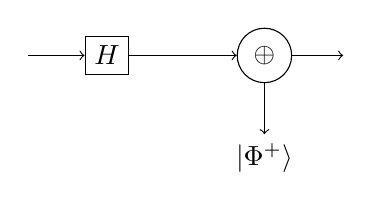
\begin{tikzpicture}
  \node[draw,rectangle] (h) at (0,0) {$H$};
  \node[draw,circle] (cnot) at (2,0) {$\oplus$};
  \draw[->] (-1,0) -- (h);
  \draw[->] (h) -- (cnot);
  \draw[->] (cnot) -- (3,0);
  \draw[->] (cnot) -- (2,-1) node[below] {$|\Phi^+\rangle$};
\end{tikzpicture}
\caption{Quantum circuit generating the Bell state $|\Phi^+\rangle$.}
\label{fig:bell_circuit}
\end{figure}

Entanglement is critical for quantum teleportation \cite{bennett1993teleporting} and enables exponential speedups in algorithms like Shor's \cite{shor1999polynomial}.

\subsection{Quantum Gates and Circuits}
\label{subsec:gates}

\begin{definition}[Quantum Gate]
A \emph{quantum gate} is a unitary operator \(U\) acting on a quantum state, meaning that \(U^\dagger U = I\). Quantum gates manipulate \glspl{qubit} and form the basic operations in quantum circuits.
\end{definition}

\begin{notation}[Single-Qubit Gates]
Key single-qubit gates include:
\begin{itemize}
    \item \textbf{Pauli-X (bit-flip):}
    \[
    X = \begin{pmatrix} 0 & 1 \\ 1 & 0 \end{pmatrix},
    \]
    which performs \(X|0\rangle = |1\rangle\) and \(X|1\rangle = |0\rangle\).
    \item \textbf{Hadamard:}
    \[
    H = \frac{1}{\sqrt{2}}\begin{pmatrix} 1 & 1 \\ 1 & -1 \end{pmatrix},
    \]
    creating superpositions as seen in the previous section.
    \item \textbf{Phase Shift:}
    \[
    R_\phi = \begin{pmatrix} 1 & 0 \\ 0 & e^{i\phi} \end{pmatrix}.
    \]
\end{itemize}
\end{notation}

\begin{definition}[Two-Qubit Gate]
A two-qubit gate, such as the \gls{cnot} gate, acts on a pair of qubits. The \gls{cnot} gate flips the second (target) qubit if the first (control) qubit is \(|1\rangle\); formally,
\[
\text{CNOT}|a\rangle|b\rangle = |a\rangle|a \oplus b\rangle,
\]
where \(\oplus\) denotes addition modulo 2.
\end{definition}

\begin{remark}
A universal set of quantum gates, for example \(\{H, T, \gls{cnot}\}\), can approximate any unitary operation to arbitrary precision, thereby forming the foundation of the quantum circuit model.
\end{remark}

\begin{example}[Deutsch-Jozsa Quantum Circuit]
Figure~\ref{fig:deutsch_circuit} shows a quantum circuit used in the Deutsch-Jozsa algorithm. The circuit demonstrates the application of Hadamard gates before and after the oracle \(U_f\), highlighting the interplay of superposition and entanglement in quantum computation.
\end{example}

\begin{figure}[h]
\centering
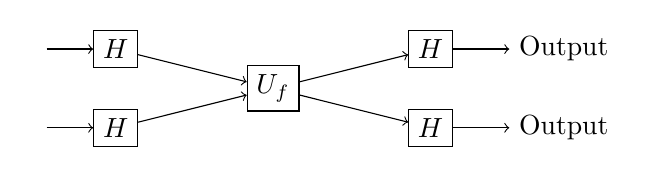
\begin{tikzpicture}[node distance=1.8cm, auto]
    \node (in1) at (0,0) {};
    \node (in2) at (0,-1) {};
    \node[draw, rectangle] (H1) at (1,0) {$H$};
    \node[draw, rectangle] (H2) at (1,-1) {$H$};
    \node[draw, rectangle] (Uf) at (3, -0.5) {\(U_f\)};
    \node[draw, rectangle] (H3) at (5,0) {$H$};
    \node[draw, rectangle] (H4) at (5,-1) {$H$};
    \draw[->] (in1) -- (H1);
    \draw[->] (in2) -- (H2);
    \draw[->] (H1) -- (Uf);
    \draw[->] (H2) -- (Uf);
    \draw[->] (Uf) -- (H3);
    \draw[->] (Uf) -- (H4);
    \draw[->] (H3) -- ++(1,0) node[right] {Output};
    \draw[->] (H4) -- ++(1,0) node[right] {Output};
\end{tikzpicture}
\caption{Quantum circuit for the Deutsch-Jozsa algorithm.}
\label{fig:deutsch_circuit}
\end{figure}

\subsection{Measurement and Probabilistic Outcomes}
\label{subsec:measurement}

Measurement in quantum mechanics is a fundamentally probabilistic process. When a quantum system in state
\[
|\psi\rangle = \sum_i \alpha_i|i\rangle
\]
is measured in the orthonormal basis \(\{|i\rangle\}\), the \textbf{Born rule} states that the outcome corresponding to \(|i\rangle\) is observed with probability
\[
P(i) = |\alpha_i|^2.
\]
This process is typically described as a \emph{projective measurement}, after which the state collapses to the observed eigenstate.

More generally, measurements can be described by \textbf{Positive Operator-Valued Measures (POVMs)}, which provide a framework for describing generalized measurements that are not necessarily projective. In a POVM, each measurement outcome is associated with a positive operator \(E_i\) satisfying \(\sum_i E_i = I\). The probability of outcome \(i\) is then given by
\[
P(i) = \langle\psi| E_i |\psi\rangle.
\]

For example, measuring the Bell state \( |\Phi^+\rangle = \frac{|00\rangle + |11\rangle}{\sqrt{2}} \) in the computational basis yields the outcomes \( |00\rangle \) or \( |11\rangle \) with 50\% probability each, as summarized in Table~\ref{tab:bell_measurement}.

\begin{table}[h]
\centering
\caption{Measurement outcomes for \( |\Phi^+\rangle \).}
\label{tab:bell_measurement}
\begin{tabular}{|c|c|}
\hline
\textbf{Outcome} & \textbf{Probability} \\ \hline
\( |00\rangle \)      & 50\%                \\ \hline
\( |11\rangle \)      & 50\%                \\ \hline
\end{tabular}
\end{table}

Measurement is an irreversible process and plays a critical role in quantum algorithms as well as in quantum automata theory, where it provides the means to extract classical information from quantum computations.

Mixed states, which describe statistical ensembles of quantum states, are represented by density matrices:
\[
\rho = \sum_i p_i |\psi_i\rangle\langle\psi_i|,
\]
with \(p_i \ge 0\) and \(\sum_i p_i = 1\). This formalism is essential when considering open systems subject to decoherence.


\subsection{Decoherence and Open Systems}
\label{subsec:decoherence}

\begin{definition}[Decoherence]
\emph{Decoherence} is the process by which a quantum system loses its coherent properties due to interaction with its environment. This results in the decay of the off-diagonal elements in the system's density matrix, leading the system to behave more classically.
\end{definition}

\begin{remark}
Decoherence is a major obstacle in quantum computing because it degrades the quantum correlations needed for quantum parallelism and entanglement.
\end{remark}

\begin{definition}[Lindblad Master Equation]
The evolution of an open quantum system can be described by the \textbf{Lindblad master equation}:
\[
\frac{d\rho}{dt} = -\frac{i}{\hbar}\,[H, \rho] + \sum_k \left( L_k \rho L_k^\dagger - \frac{1}{2}\{L_k^\dagger L_k, \rho\} \right),
\]
where \(\rho\) is the density matrix, \(H\) is the Hamiltonian, and \(L_k\) are the Lindblad (noise) operators \cite{breuer2002theory}.
\end{definition}

\begin{example}[Noise Models]
    Typical noise models include:
    \begin{itemize}
        \item \textbf{Amplitude damping}: Models energy loss (e.g., spontaneous emission) \cite{nielsen2010quantum}.
        \item \textbf{Phase damping}: Represents the loss of phase coherence without energy dissipation \cite{nielsen2010quantum}.
    \end{itemize}
\end{example}

\begin{observation}
    To combat decoherence, quantum error correction codes (such as the Shor code \cite{shor1995scheme} and surface codes \cite{fowler2012surface}) and decoherence-free subspaces are employed.
\end{observation}
 
\subsection{Unitary Evolution and Quantum Dynamics}
\label{subsec:unitary_evolution}

\begin{definition}[Unitary Evolution]
In a closed quantum system, the state evolution is governed by the Schrödinger equation,
\[
i\hbar \frac{d}{dt} |\psi(t)\rangle = H |\psi(t)\rangle,
\]
where \(H\) is the Hamiltonian. The solution to this equation is given by
\[
|\psi(t)\rangle = U(t)|\psi(0)\rangle, \quad \text{with } U(t)=e^{-iHt/\hbar},
\]
where \(U(t)\) is a unitary operator.
\end{definition}

\begin{remark}
Unitary evolution is reversible and forms the basis for the operation of quantum circuits, where continuous evolution is discretised into sequences of quantum gates.
\end{remark}

\begin{theorem}[No-Cloning Theorem]
    Let \(\mathcal{H}\) be a Hilbert space with \(\dim \mathcal{H} \ge 2\). There is no unitary operator \(U\) such that for all states \(|\psi\rangle \in \mathcal{H}\) the following holds \cite{wootters1982single}:
    \[
    U\big(|\psi\rangle \otimes |0\rangle\big) = |\psi\rangle \otimes |\psi\rangle
    .\]
\end{theorem}

\begin{observation}
    The \textbf{no-cloning theorem} states that it is impossible to create an exact copy of an arbitrary unknown quantum state. This fundamental principle has significant implications for quantum information processing and quantum cryptography.
    The no-cloning theorem ensures that quantum information cannot be perfectly replicated, which underpins the security of many quantum cryptographic protocols such as BB84 \cite{bennett1984quantum}.
\end{observation}    

\subsection{Summary}
\label{subsec:quantum_summary}

The foundations of quantum mechanics—qubits, superposition, entanglement, unitary evolution, measurement, and decoherence—form the bedrock upon which quantum automata theory is built. Understanding these principles is crucial for grasping how quantum automata differ from their classical counterparts and how quantum effects can be harnessed to achieve computational advantages.
